% Flujo de datos: de los archivos de SIATA a la tabla supervisada.
% Cifras de notebooks/01_eda_pm25.ipynb y notebooks/02_modelado.ipynb.
\documentclass[border=2pt]{standalone}
% Estilo común de los diagramas: letra sin serifa, como las figuras del
% notebook, y ancho máximo de una columna IEEE (8,9 cm). Compilar con pdflatex.
\usepackage[utf8]{inputenc}
\usepackage[T1]{fontenc}
\usepackage{tgheros}
\renewcommand{\familydefault}{\sfdefault}
\usepackage{tikz}
\usetikzlibrary{positioning, arrows.meta, fit, backgrounds, calc}

\definecolor{pm}{HTML}{1F77B4}
\definecolor{meteo}{HTML}{2CA02C}
\definecolor{modelo}{HTML}{FF7F0E}
\definecolor{perdida}{HTML}{B22222}
\definecolor{gris}{HTML}{6E6E6E}

\tikzset{
  caja/.style={draw=#1, fill=#1!8, rounded corners=2pt, line width=0.6pt,
    align=center, inner sep=3pt, font=\fontsize{6.5}{7.8}\selectfont},
  caja/.default=gris,
  flecha/.style={-{Stealth[length=4pt]}, line width=0.6pt, draw=gris},
  nota/.style={font=\fontsize{5.8}{7}\selectfont, text=perdida, align=left},
  titulo/.style={font=\fontsize{6.5}{7.8}\selectfont\bfseries, text=#1},
}
\newcommand{\menos}[1]{\textcolor{perdida}{\fontsize{5.8}{7}\selectfont #1}}


\begin{document}
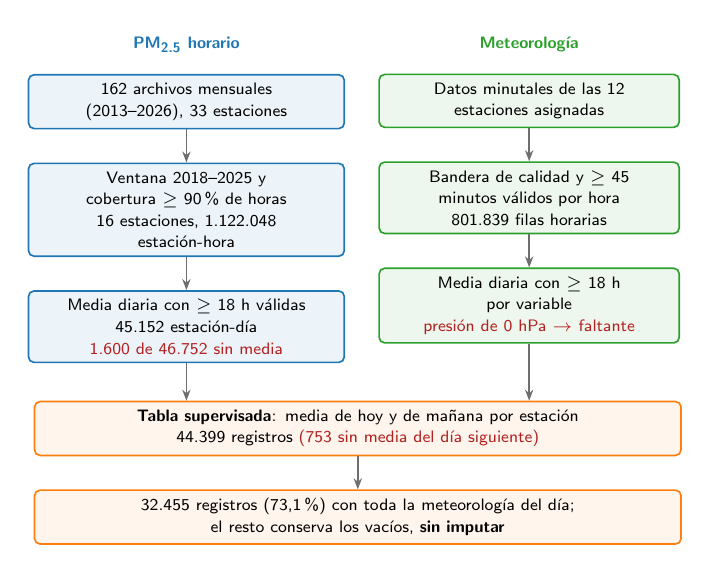
\begin{tikzpicture}[node distance=4.2mm]
  \node[titulo=pm] (tpm) {PM\textsubscript{2.5} horario};
  \node[caja=pm, text width=38mm, below=1.5mm of tpm] (a)
    {162 archivos mensuales\\(2013--2026), 33 estaciones};
  \node[caja=pm, text width=38mm, below=of a] (b)
    {Ventana 2018--2025 y\\cobertura $\geq$ 90\,\% de horas\\
     16 estaciones, 1.122.048\\estación-hora};
  \node[caja=pm, text width=38mm, below=of b] (c)
    {Media diaria con $\geq$ 18 h válidas\\45.152 estación-día\\
     \menos{1.600 de 46.752 sin media}};

  \node[titulo=meteo, right=44mm of tpm.west, anchor=west] (tme) {Meteorología};
  \node[caja=meteo, text width=36mm, below=1.5mm of tme] (m1)
    {Datos minutales de las 12\\estaciones asignadas};
  \node[caja=meteo, text width=36mm, below=of m1] (m2)
    {Bandera de calidad y $\geq$ 45\\minutos válidos por hora\\801.839 filas horarias};
  \node[caja=meteo, text width=36mm, below=of m2] (m3)
    {Media diaria con $\geq$ 18 h\\por variable\\
     \menos{presión de 0 hPa $\to$ faltante}};

  \node[caja=modelo, text width=80mm, below=6mm of $(c.south)!0.5!(m3.south)$] (d)
    {\textbf{Tabla supervisada}: media de hoy y de mañana por estación\\
     44.399 registros \menos{(753 sin media del día siguiente)}};
  \node[caja=modelo, text width=80mm, below=of d] (e)
    {32.455 registros (73,1\,\%) con toda la meteorología del día;\\
     el resto conserva los vacíos, \textbf{sin imputar}};

  \draw[flecha] (a) -- (b);
  \draw[flecha] (b) -- (c);
  \draw[flecha] (m1) -- (m2);
  \draw[flecha] (m2) -- (m3);
  \draw[flecha] (c.south) -- (c.south |- d.north);
  \draw[flecha] (m3.south) -- (m3.south |- d.north);
  \draw[flecha] (d) -- (e);
\end{tikzpicture}
\end{document}
